\documentclass[a4paper,12pt]{article}
\usepackage[utf8]{inputenc}
\usepackage[spanish]{babel}
\usepackage{framed, color}
\usepackage{textcomp}
\usepackage{vmargin}
\usepackage{graphicx}
\usepackage[table,xcdraw]{xcolor}
\usepackage{enumerate} % enumerados

%--------Codigos para tipos de letras%---------------
\usepackage[T1]{fontenc}
\usepackage{pdfpages}
\usepackage[bitstream-charter]{mathdesign} 
\usepackage{textcomp} %Paquete para algunos caracteres especiales

\setpapersize{A4}
\setmargins
{2.5cm}          % margen izquierdo
{1.5cm}          % margen superior
{16.5cm}         % anchura del texto
{23.42cm}        % altura del texto
{10pt}           % altura de los encabezados
{1cm}            % espacio entre el texto y los encabezados
{0pt}            % altura del pie de página
{2cm}            % espacio entre el texto y el pie de página
\usepackage{titlesec}
\setcounter{secnumdepth}{4}
\titleformat{\paragraph}
{\normalfont\normalsize\bfseries}{\theparagraph}{1em}{}
\titlespacing*{\paragraph}
{0pt}{3.25ex plus 1ex minus .2ex}{1.5ex plus .2ex}
\begin{document}
	\begin{titlepage}
		\begin{center}
			\vspace*{0.8in}
			\begin{figure}
				\centering
				
\includegraphics[width=0.9\linewidth]{graficos/unalogos.jpg}
				UNIVERSIDAD NACIONAL DE ASUNCIÓN\\
				\vspace*{0.15in}
				FACULTAD POLITÉCNICA\\
			\end{figure}
			\begin{large}
				\textbf{Maestría en Tecnologías de la Información y Comunicación}\\
				\vspace*{0.3in}
				\textbf{Ingeniería de Software}\\
				\textbf{Propuesta de tema de Tesis}\\
			\end{large}
			\vspace*{0.6in}
			\begin{Large}
				\textbf{ENFOQUE DE MINERÍA DE DATOS PARA EL ESTUDIO DE GATOS SALARIALES DEL MINISTERIO DE HACIENDA} \\
			\end{Large}
			\vspace*{0.3in}
			\rule{80mm}{0.1mm}\\
			\vspace*{0.4in}
			\begin{large}
				\textbf{Tutor:} Msc. Santiago Gómez\\
				\vspace*{0.3in}
				\textbf{Autor:} Mario Asunción Cañiza  Páez\\mario.caniza@gmail.com\\
				\vspace*{0.6in}
				Agosto - 2.017
				\vspace*{0.20in}
			\end{large}
		%\local{Fortaleza -- Ceará}
		\end{center}
	\end{titlepage}
%	\tableofcontents
	\newpage
%	\listoffigures
%	\newpage
%	\listoftables
	\newpage
	\section{PROPUESTA}
Enfoque de minería de datos para el estudio de gastos salariales del Ministerio de Hacienda.

\section*{RESUMEN}
En una institución pública se procesan grandes cantidades de datos y se genera mucha información, pero las mismas no pueden ser analizadas ni utilizadas en su plenitud con las técnicas tradicionales. Utilizando y aplicando técnicas de minería de datos nos ayudará a obtener conocimiento valedera para predecir el futuro, a tomar decisiones y lo mas importante ayudará a comprender mejor el entorno.\\

En este trabajo se estudiará el tratamiento de dichos datos estadísticos de ingresos y egresos varios de los funcionarios, se aplicarán técnicas de minería de datos para generar información oportuna que brindará conocimientos sobre problemas y causas, a los niveles superiores administrativos, sobre la situación financiera de sus subalternos con el fin de fortalecer áreas vulnerables.\\

\section{OBJETIVOS}
\subsection{OBJETIVO GENERAL}
Aplicar técnica de minería de datos para el estudio de gastos salariales del capital humano del Ministerio de Hacienda.
\subsection{OBJETIVOS ESPECÍFICOS}
\begin{itemize}
	\item
	Comparar la estructura salarial actual frente al mercado laboral actual.
	\item
	Identificar niveles de endeudamientos del funcionariado.
	\item
	Estudiar el aumento de gastos salariales de funcionarios con años anteriores.
	\item
	Predicción de gastos para la planificación presupuestaria.
	\item
	Análisis mensual de las multas aplicadas al personal.
	\item
	Conocer gastos salariales del personal contratado por tipo de contrato.
	\item
	Comparación de ausentismo laboral entre determinados periodos.
	\item
	Índice de ejecución del presupuesto salarial más presupuesto contratos comparado con índice de ejecución presupuestaria global.
	\item
	
\end{itemize}

\section{APORTE INNOVADOR DEL TRABAJO}
Con la realización de este trabajo lo que se pretende es buscar una herramienta que proporcione informaciones estadísticos de los gastos públicos en lo que refiere a pago de salarios al personal, para la toma de decisiones, a fin de mejorar los procesos y las condiciones de vida laboral del capital humano.\\

Esta investigación beneficiará a la institución ya que se extraerán informaciones con que se cuenta, desde distintas perspectivas, con el objetivo de resumir datos en fuentes de informaciones útiles. Esta información podrá ser utilizada para incrementar beneficios, reducir gastos, conocer el estado del personal que presta servicio.
\section{CRONOGRAMA TENTATIVO}

%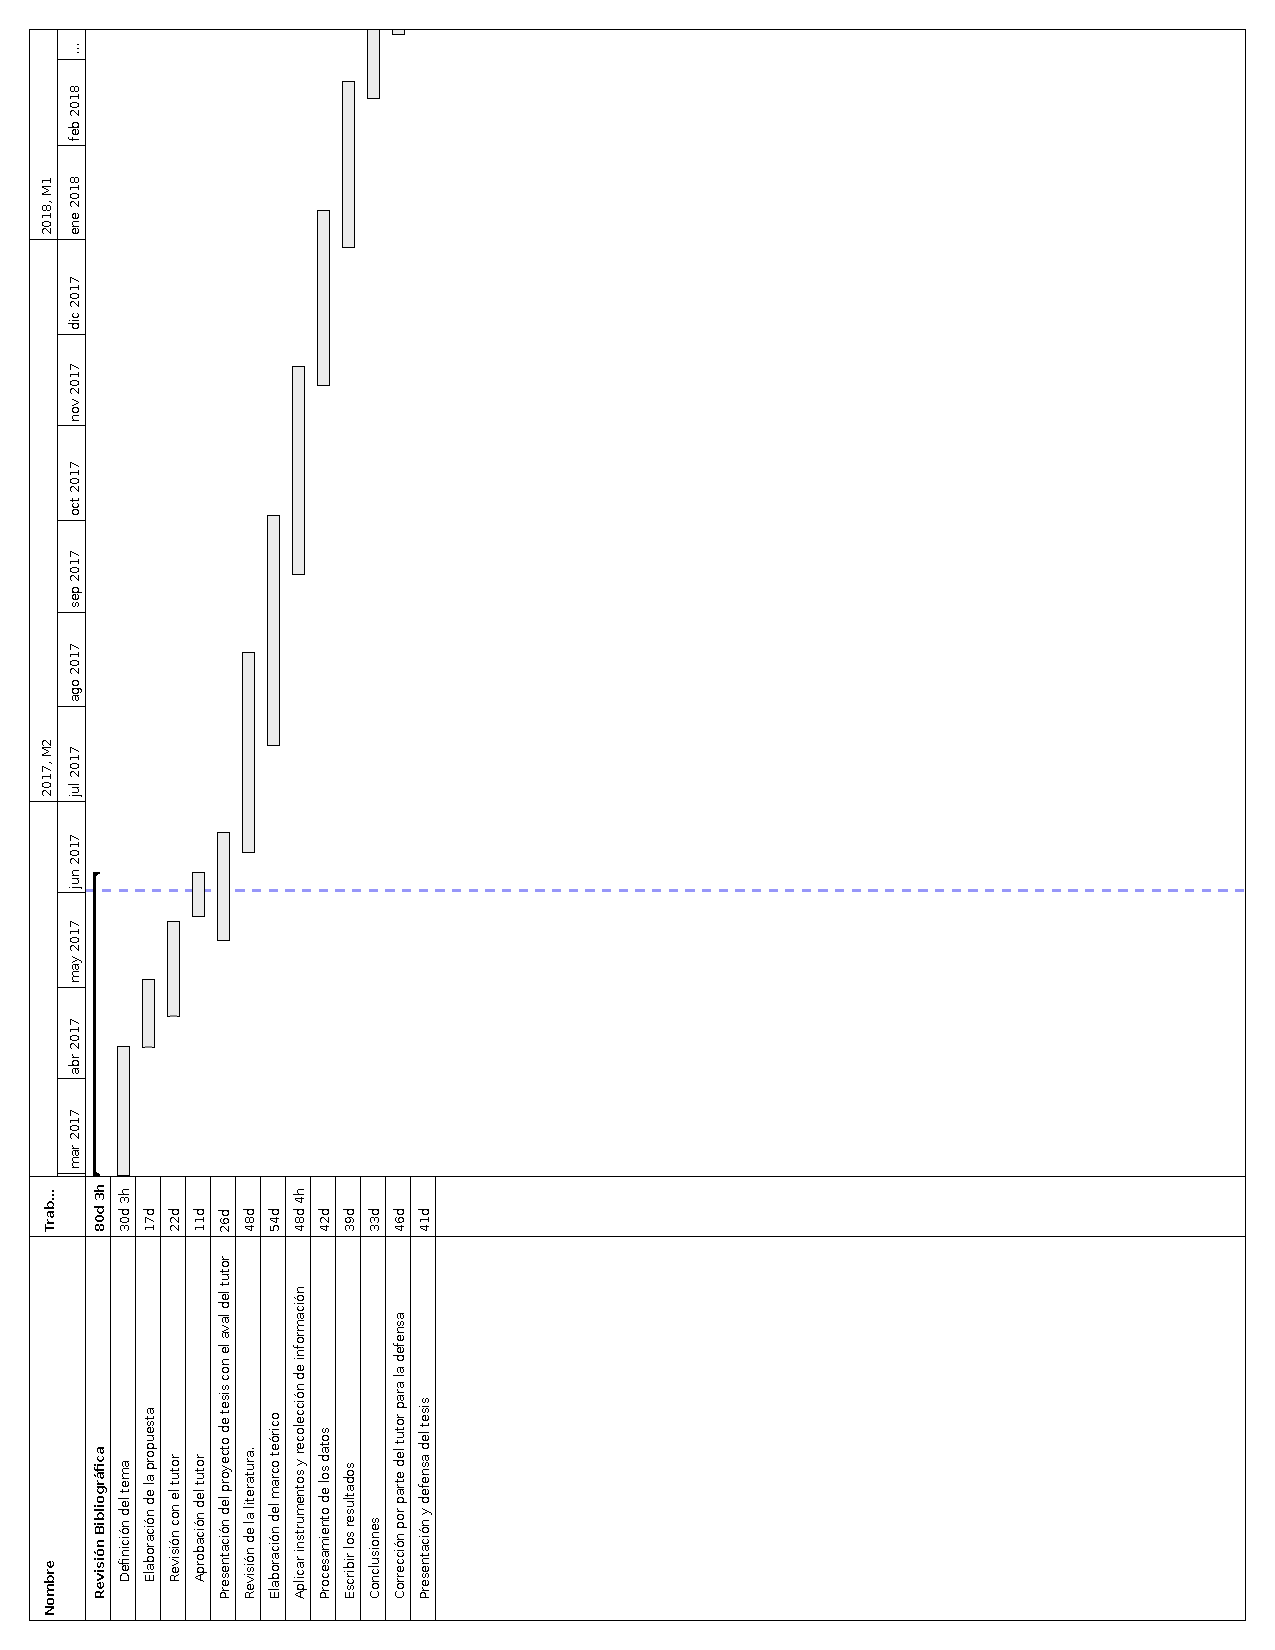
\includepdf[pages=1]{gantt}
%\newpage
 \setlength{\parindent}{2cm}

\begin{table}[htbp]
	\centering
	%\caption{My caption}
	\label{my-label}
	\begin{tabular}{cc}
		------------------------------------------------------ & ------------------------------------------------------ \\
		Mario Asunción Cañiza Páez                             & Msc. Santiago  Gómez                                      \\
		Firma del alumno                                       & Firma del tutor                                       
	\end{tabular}
\end{table}



	%\section*{ÁREA DE INVESTIGACIÓN}
	%\section*{RESUMEN DEL TRABAJO}
	%\section*{OBJETIVOS}
	%\section*{APORTE DE LA INVESTIGACIÓN}
	%\section*{CRONOGRAMA}
	\end{document}